\chapter{评估}
在本节中,我们进行全面评估以回答以下问题:
• RQ1:LLMalMorph 生成的恶意软件变体对广泛使用的防病毒引擎和机器学习分类器的检测具有多强的抗性?其规避能力与最近的对抗性恶意软件生成框架生成的变体相比如何?
• RQ2:不同转换策略间的代码编辑工作量有何差异?这对揭示 LLM 所犯错误类型有何启示?
• RQ3:生成的恶意软件变体是否保留了原始样本的语义和功能?

\section{评估设置}

\subsection{选择样本}
由于最新的恶意软件源代码稀缺,大多数恶意软件研究都集中在可执行文件上。我们检查了公共数据库 \parencite{Cryptware2024}, \parencite{Vxunderground2024},发现大多数可用的 Windows 恶意软件源代码是 32 位的,因此我们将研究重点放在 32 位变体上。我们选择了能够编译成可运行可执行文件、并表现出可通过 VirusTotal 或 Hybrid Analysis 检测到的恶意行为(其 AV 检测率≥60\%)的样本。这产生了十个具有不同复杂性和类型的恶意软件候选样本。RansomWar 样本使用 GCC 编译,其余样本使用 Microsoft Visual Studio 2022\footnote{https://visualstudio.microsoft.com/vs/}编译(因为提供了 .sln 文件)。表 II 总结了选定样本的关键细节。对于 Conti 和 Babuk 勒索软件,我们的分析集中在负责加密的加密器组件上。有关样本的详细信息请参见附录 B。

\subsection{评估指标}
我们使用给定的评估指标:防病毒(AV)检测率($R^{\hat{Ms}}$)。我们使用 VirusTotal 评估 AV 检测率,该平台使用来自不同供应商的多个 AV 引擎扫描样本。每个样本可用的检测器数量因可用性而异。令 $D$ 为可用检测器的集合,$\hat{D} \subseteq D$ 为将恶意软件变体标记为恶意的检测器集合。在第 k 次运行时,变体 $\hat{M_{s}}$ 的 AV 检测率 $R^{\hat{M_{s}}}_{k}$ 定义为 $R^{\hat{M_{s}}}_{k} = \frac{|\hat{D}|}{|D|} \times 100$,其中 $|.|$ 表示两个集合的大小。

每个样本将进行$k$次运行,并计算平均检测率$R^{\hat{M_{s}}}=\frac{1}{k} \sum_{i=1}^{k} R_{k}^{\hat{M_{s}}}$。我们在实验中设定 k=3 以解释不同运行间的变异性。我们还使用 Hybrid Analysis,该工具包含静态分析、基于机器学习的分析以及使用不同引擎的多重扫描分析。检测性能以每个恶意软件样本及其变体在 k 次运行上的平均百分比表示。我们使用这两个工具的免费版本,并通过其各自的 API 自动化样本上传、结果检索和后处理。

\subsection{策略导向的机器学习分类器攻击成功率 (ASR)}
攻击成功率 (Attack Success Rate, ASR) 是评估对抗攻击的广泛使用的指标\parencite{Lucas2021}, \parencite{Ling2019},即生成的恶意软件变体成功逃避目标系统检测的比例。我们针对三种基于机器学习的恶意软件分类器评估 ASR:Malconv\parencite{Raff2017}、Malgraph\parencite{Ling2022} 和一个训练好的 ResNet50 恶意软件分类\parencite{Li2025}。模型细节详见附录 E。令 M 为一个原始恶意软件样本,将我们的策略 s 应用于所有修改文件 $\hat{F} \subseteq F$ 并为 $j$ 个转换函数生成变体 $V_{s}^{M} = \{\hat{M_{1}}, \hat{M_{2}}, ..., \hat{M_{j}}\}$。对于给定的目标分类器 $C$,令 $\hat{V_{s,C}^{M}} = \{ \hat{M} \in V_{s}^{M} : C(\hat{M}) = benign\}$ 为成功逃避 $C$ 的变体子集。则攻击成功率为 $ASR = \frac{|\hat{V_{s,C}^{M}}|}{|V_{s}^{M}|} \times 100$。其中 $|.|$ 表示集合的大小。

\subsection{策略导向的代码编辑工作量 ($W_{s}^{M}$)}
该指标基于需要手动编辑以编译LLM生成代码的总代码行数来比较策略 $s$。值越高表明需要更广泛的手动干预,意味着LLM在该策略下犯了更严重的错误。对于给定的恶意软件 $M$,令 $\hat{F} \subseteq F$ 表示 $F$ 个文件中被修改的文件数量。恶意软件 $M$ 和策略 $s$ 的编辑工作量 $W_s^{M}$ 定义为在文件 $\hat{F}$ 中所有转换后的函数 $\{f_{1}^{i}, f_{2}^{i}... f_{j}^{i}\}$ 上编辑(添加、修改或删除)的总代码行数,计算公式为 $W_{s}^{M}=\sum_{i=1}^{\hat{F}} \sum_{t=1}^{j} L_{edit}(f_{t}^{i})$,其中 $L_{edit}$ 统计函数 $\hat{f_{t}^{i}}$ 被编辑代码的行数。

\subsection{人力投入量化指标 ($H_{s}^{M}$)}
该指标衡量针对每种策略调试和配置恶意软件中转换后函数所需的人力投入。它量化了生成一个成功编译的 PE 文件所需的总工时。对于给定的恶意软件 $M$ 和代码转换策略 $s$,人力投入 $H_{s}^{M}$ 的计算公式为 $H_{s}^{M} = \sum_{i=1}^{\hat{F}} \sum_{t=1}^{j} ManHours(\hat{f_{t}^{i}})$。此处,求和表示在策略 $s$ 下,在修改文件 $\hat{F}$ 中所有转换后的函数 $\{f_{1}^{i},f_{2}^{i}...f_{j}^{i}\}$ 上所花费的总工时。

\subsection{功能保留指标 ($\Phi^{M}$)}
该指标评估了经 LLMalMorph 转换后,恶意软件语义在变体中保留的程度。由于可执行文件固有的复杂性,尚无精确方法能判断恶意软件 $M$ 与其变种 $\hat{M}$ 之间的语义等价性 \parencite{Apel2009}。因此,文献中遵循的评估方法包括比较恶意软件与其变体之间的 API 调用序列 \parencite{Ling2024},或通过在沙箱中运行来比较恶意软件及其变体的行为\parencite{Lucas2021}, \parencite{Digregorio2024}。

我们采用类似方法,并利用最长公共子序列 (lcs) 算法来比较 $M$ 和 $\hat{M}$ 之间的 API 调用序列。转换后的变体必须保留原始的 API 调用顺序,允许存在不破坏此序列的额外调用。API 调用序列使用专有沙箱收集。归一化的最长公共子序列定义为 $\hat{lcs}(M, \hat{M})= \frac{lcs(M, \hat{M})}{Length(API(M))}$,其中分母是 $M$ 的 API 序列长度。分数范围从 0 到 1,1 表示完全相同的 API 序列。最后,我们计算功能保留率 $\Phi^{M} = \frac{|\hat{M} \in \psi^{\hat{M}}:\hat{lcs}(M,\hat{M}) \geq \delta|}{|\psi^{\hat{M}}|} \times 100$。

此处,$\psi^{\hat{M}}$(总变体集)定义为所有 AV 检测率 $R^{\hat{M_{s}}}$ 低于 $M$ 的基线检测率的恶意软件变体 $\hat{M}$ 的集合。分子代表 $\psi^{\hat{M}}$ 中保留了语义等价性的子集的大小,我们通过考虑归一化的最长公共子序列得分(其值大于预定义阈值 δ)来确定该子集,而 $|\psi^{\hat{M}}|$ 是整个总变体集的大小。我们通过经验分析恶意软件变体和原始样本,选择 $\delta$ 的值为 0.96。我们选取不同样本在离散值集上的恶意软件变体,并将其上传到 Triage Sandbox\footnote{https://tria.ge/}。我们分析了变体和原始恶意软件样本的报告,以比较行为指标、注册表修改、网络调用等。我们观察到,在某些情况下,行为漂移在分数低于 0.96 时开始出现,而在其他情况下,即使分数略高于该值,功能等价性也得以保持。然而,大多数保留了关键行为的变体得分在 0.96 或以下。因此,我们选择 $\delta = 0.96$ 作为上限,以确保被接受的变体在 API 序列和执行行为上保持高度相似性。

\section{模型选择}
虽然 LLMalMorph 可以利用任何 LLM 生成恶意软件变体,但我们选择 Codestral-22B \parencite{MAI2024} 作为我们的主要 LLM。我们精心设计的提示包含许多需要遵循的约束和指示。我们观察到 Codestral 模型能够比其他模型更精确地遵循这些特定指令来变异函数。此外,Codestral 为我们的用例提供了一组均衡的特性——220 亿参数、12 GB 模型大小和 32K 上下文窗口——并且与具有更高硬件要求的模型相比,它在长距离仓库级代码补全任务上具有卓越性能 \parencite{Dubey2024}, \parencite{Roziere2023}。

\section{实现细节}
在 LLMalMorph 中,Function Mutator 内的 Extractor 子模块使用 Tree-sitter Parser\footnote{https://tree-sitter.github.io/tree-sitter/} 的 Python 绑定实现,利用其基于 C 的运行时进行高效解析。对于 LLM,我们使用了 Ollama\footnote{https://ollama.com/},它便于本地 LLM 执行而无需外部 API 依赖,并提供了一个基于 Python 的接口。我们的实验设置包括一台配备 252 GB RAM 和 48 个处理器的 RTX 3090 GPU 服务器,以及一台配置了 VirtualBox\footnote{https://www.virtualbox.org/} 用于恶意软件编译的 Windows 10 虚拟机。LLMalMorph 的核心实现主要使用 Python 开发,部分组件(例如基于 lcs 的语义指标计算)使用 C++ 实现。

\section{评估结果与分析}
我们使用算法 \ref{alg:Function Transformation Using LLM} 和 \ref{alg:Malware Variant Generation} 对要修改的文件进行优先级排序,按函数数量升序排列。这假设对源代码了解有限的攻击者会针对函数较少的文件,以最小化工作量并最大化修改文件的数量。如果出现平局,则随机选择文件。我们依次修改每个文件内的函数,但这可能会忽略对恶意软件行为至关重要的关键函数。自动化分离恶意函数具有挑战性,因为看似良性的函数(例如,简单的线程管理)可能促成恶意活动。我们的目标是评估这种简单的顺序方法是否能在不损害功能的情况下产生规避性变体。有关文件选择标准以及每个样本选择要修改的函数数量的标准,请参见附录 C。

\subsection{对研究问题1(RQ1)的解答}
我们评估了恶意软件变种逃避杀毒软件检测器的有效性。图\ref{fig:5.1}与图\ref{fig:5.2}展示了10个恶意软件样本在VirusTotal和Hybrid Analysis平台的检测率。六种代码转换策略以不同颜色标注,标记点表示被修改的文件。每个数据点代表特定策略的检测率;x轴按递增顺序显示被修改的函数数量(例如3代表函数1–3),y轴则绘制杀毒软件检测率($\hat{R}_k^{M_{s}}$)。黑色虚线标示各样本的基准检测率,红色虚线显示所有变种的平均检测率。此外,我们展示了针对Malgraph分类器的四个样本通过不同策略实现的攻击成功率(ASR),并简要讨论了与最新对抗性恶意软件生成框架的对比分析。

%begin picture
\begin{figure}[htb]
	\centering
	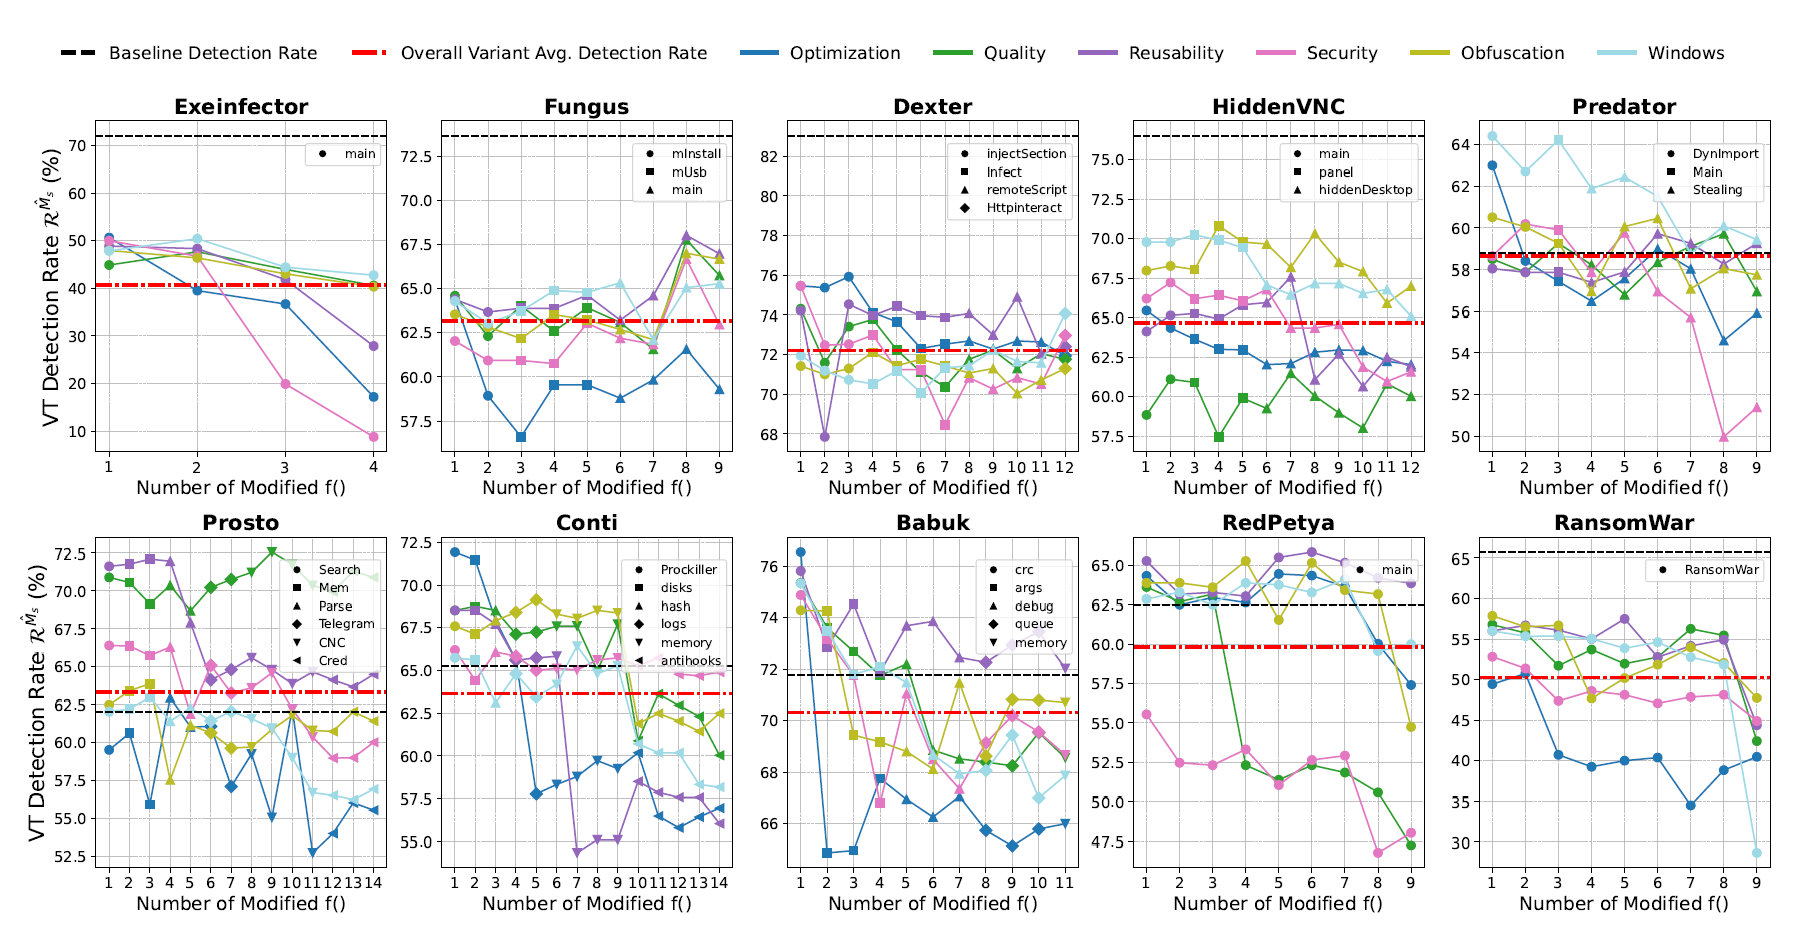
\includegraphics[width=1.15\textwidth]{figures/figure2_a.png}
	\caption{VirusTotal和混合分析对十个恶意软件样本采用不同策略的检测率比较-VirusTotal检测率}
	\label{fig:5.1}
\end{figure}
\begin{figure}[htb]
	\centering
	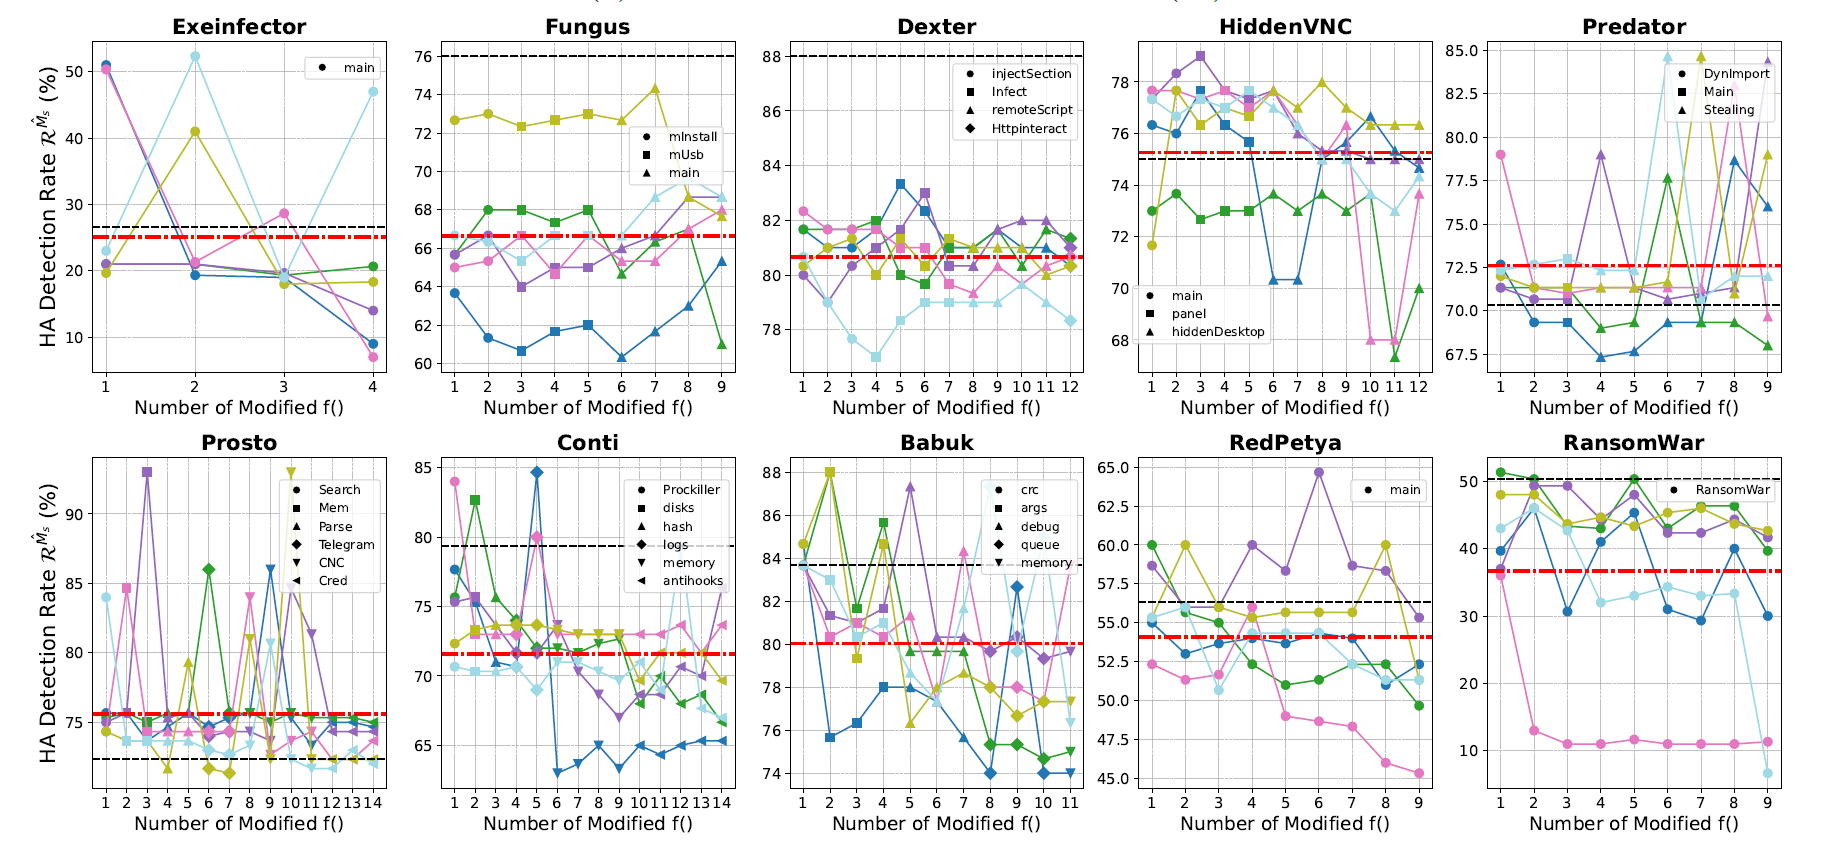
\includegraphics[width=1.15\textwidth]{figures/figure2_b.png}
	\caption{VirusTotal和混合分析对十个恶意软件样本采用不同策略的检测率比较-混合分析检测率}
	\label{fig:5.2}
\end{figure}

\subsection{VirusTotal}
图\ref{fig:5.1}显示,10个样本中有5个样本的所有恶意软件变种检测率均低于各自基准值。对于Exeinfector,其变种平均检测率为40.708\%,比基准值72.009\%低31.301\%,且检测率呈下降趋势。最显著的下降发生在修改第4个函数后,此时Reusability、Optimization和Security策略的检测率均跌破30\%,较基准值下降超42\%。在Fungus样本(第2个子图)中,平均检测率为63.167\%,而基准值为73.630\%。Optimization策略在修改三个函数(包括文件mUsb中操纵USB驱动器创建隐藏目录并自动执行文件的第三个函数)后达到最低检测率56.611\%。在图\ref{fig:5.1}的Dexter子图中,检测率平均值为72.211\%,比基准值83.020\%低10.809\%。该样本的详细数据见附录D。对于HiddenVNC样本,平均检测率为64.664\%,较基准值76.503\%低11.84\%。Optimization与Quality变种检测率持续较低,而Security与Windows变种呈下降趋势;Reusability策略在第7次至第8次函数修改期间从67.593\%显著降至61.081\%。被修改的第八个函数被拆分为六个更小的函数,用于枚举可见窗口并捕获其内容。

对于Predator样本,平均检测率与基准值几乎相同,多数变种表现相似。但Security策略呈下降趋势,其在第8个函数处达到最低检测率49.967\%(较基准值低8\%),Optimization策略紧随其后为54.591\%。Prosto样本的详细数据见附录D。在Conti勒索软件样本中,大多数变种检测率接近65.275\%的基准值,但Reusability策略在第7个函数处出现大幅下降,Optimization策略在第5个函数处同样大幅下跌——二者起始高于基准值但之后持续低于该值。Windows策略与Quality策略亦呈现下降趋势。对于Babuk样本,多数策略的检测率出现中等程度下降,其中Optimization策略在早期阶段造成最显著的跌幅。详细分析见附录D。

对于RedPetya样本,我们观察到Security与Quality变种的检测率呈下降趋势。值得注意的是,Security策略在第8个函数处出现最急剧下降至46.746\%,较基准值降低15.75\%。该下降源于LLM使用了替代OpenSSL的加密库。被修改的第8个函数$hard\_reboot$通过调用Windows API调整进程权限并触发重启,使勒索软件能在下次启动时重获控制权,这是关键持久化机制。在RansomWar样本中,50.251\%的平均检测率较65.728\%的基准值低15.478\%,所有变种均跌破基准值。多数变种检测率位于50-58\%区间,而Optimization策略在第3个函数修改后跌至34.5\%。Windows策略以28.651\%的检测率(低于基准值37\%)达到最低值,展现出强规避能力。

整体而言,Optimization策略在降低恶意软件检测率方面表现最为稳定,其次为Security与Reusability策略,而Windows策略虽在各样本中展现出强规避能力但效果波动较大。Optimization策略通过引入和重组数据结构,结合可能改变控制流与数据流的特定语言特性,从而修改了杀毒引擎通常可检测的代码模式与语义。这些特定修改需要新增头文件及库引用,进而引发编译后二进制文件的变化,最终改变其在杀毒检测器中的识别蓝图。Security策略采用替代性加密库可导致更显著的二进制差异,破坏杀毒软件基于模式的启发式签名机制,从而产生低于基准值的检测率。

\subsection{混合检测}
在图\ref{fig:5.2}的Exeinfector子图中,Optimization与Security策略在第二次函数修改后呈现下降趋势。混淆策略在修改第二个函数后将检测率提升至41\%,这可能源于引入了已知的反调试函数。类似地,Windows策略在两次及四次修改后显示更高检测率,表明LLM生成的替代性API调用更易被检测到。在HiddenVNC的第四个子图中,Quality策略对第10个函数添加错误检查后达到最低检测率67.333\%。Security策略中,添加到第10个函数的基于OpenSSL的功能会暂时降低检测率,之后出现回升;Optimization子图也观察到类似情况。在第二个Fungus子图中,所有变种的平均检测率为66.636\%,较76\%的基准值低9.364\%,其中Optimization策略实现最低检测率并生成最具规避性的变种。对于Dexter样本,88\%的基准检测率降至80.653\%的平均值。Windows策略在四次函数修改后达到最低检测率,这些修改涉及LLM生成的代码转换,包括替换基于注册表修改的函数,以及使用$ZeroMemory()$和$lstrlenA()$实现安全内存处理与字符串长度计算。

对于第5至第9个子图,检测率出现骤升现象,这是因为Hybrid Analysis有时跳过杀毒软件检测环节,仅依赖机器学习与静态分析,导致分数虚高(例如100/90)并扭曲平均值。Predator与Prosto样本整体变化极小,而Conti样本出现显著的Optimization策略特异性下降;这三个子图(5-7)的详细分析见附录D。在Babuk样本中,Optimization策略持续降低检测率,最低达74\%,较基准值83.667\%下降约10\%,该趋势与图\ref{fig:5.1}一致。Quality与Obfuscation策略同样呈现下降趋势。对于RedPetya样本,Security策略在第9个函数处降至45.333\%,在第8个函数处为46.0\%,与图\ref{fig:5.1}趋势一致,证明LLM在函数转换中的有效性。在RansomWar样本中,变种平均检测率36.697\%较基准值50.333\%低13.636\%。Security策略保持稳定的10\%检测率,而Windows策略以6\%的检测率达到最低值,较基准下降44\%。

这些发现印证了VirusTotal的结果:Optimization、Security与Windows策略对降低检测率贡献最大。如前所述,Optimization策略可能重塑控制流与数据流,而Security策略采用替代性加密库会向修改后的恶意软件二进制文件引入新导入项和符号。这不仅影响基于签名的检测器,也可能影响混合检测使用的静态与机器学习检测器。值得注意的是,对于两个检测平台,检测率下降程度与被修改函数的数量无关,且可能产生相反效果。

\subsection{机器学习分类器}
\begin{table}[htbp]
	\centering
	\caption{各策略的 ASR(\%)。百分比已对不同变体数量进行标准化(Fungus:9 个变体/策略;Dexter:12 个;Conti:14 个;Babuk:11 个)。}
	\label{tab:5.1}
	\begin{tabular*}{\textwidth}{@{\extracolsep{\fill}}ccccccc}
		\toprule
		样本 & Optimization & Quality & Reusability & Security & Obfuscation & Windows \\
		\midrule
		Fungus & 88.889 & 0 & 11.111 & 0 & 0 & 0 \\
		Dexter & 50.00 & 16.667 & 0 & 41.667 & 33.333 & 0 \\
		Conti & 71.429 & 0 & 0 & 0 & 0 & 0 \\
		Babuk & 0 & 72.727 & 0 & 90.909 & 0 & 0 \\
		\bottomrule
	\end{tabular*}
\end{table}

针对每个ML模型,我们选择其对应的0.1\%误报率(FPR)阈值作为检测阈值。Malconv与ResNet50模型未将原始10个样本中的任何样本识别为恶意软件,而Malgraph仅标记了Fungus、Dexter、Conti和Babuk样本。因此我们仅展示这四个样本在Malgraph上的检测结果。阈值设定细节详见附录E,攻击成功率(ASR)数据列于表\ref{tab:5.1}:

第一列列出四个样本名称,后续列展示六种转换策略的攻击成功率(ASR)。Optimization策略在第一和第三样本中实现高ASR,在第二样本中取得中等成功率;Security策略在Babuk样本呈现高成功率,在Dexter样本为中等成功率,这与杀毒检测器的观测结果一致。Babuk样本在Quality策略下同样表现出显著成功率,与其在Hybrid Analysis(图\ref{fig:5.2})中的行为一致。Reusability与Obfuscation策略在两个样本中成功率较低,而Windows策略未能规避检测。


尽管LLMalMorph通过提示词工程和精选转换策略修改函数(未直接针对任何ML恶意软件分类器进行优化),仍在部分样本的Optimization与Security等策略上展现出显著ASR,这支持了杀毒检测率降低的观测结论。正如先前在杀毒检测器语境中指出的,这些策略的高ASR可能源于LLM使用新库、新特性及控制流重组,这些改变很可能促进了规避成功。

\subsection{比较分析}
现有大多数对抗性恶意软件生成研究(包括Malguise\parencite{Ling2024}等最新框架)集中于直接修改已编译的二进制文件以生成规避性变种。因此,我们将LLMalMorph与领先的二进制级对抗性恶意软件生成框架Malguise进行对比。如研究问题1(RQ1)解答中机器学习分类器小节所述,仅有4/10样本(Fungus、Dexter、Conti和Babuk)被Malgraph分类器识别为恶意软件,其他分类器没有任何样本被判定为恶意。我们在上述四个样本上运行Malguise\parencite{Ling2024},以Malgraph为规避目标,为每个样本生成对抗性变种。Fungus、Dexter和Babuk成功绕过Malgraph分类器,而Conti未能实现规避。尽管如此,我们收集了Malguise生成的所有对抗性变种(三个成功规避样本和一个未成功样本),通过VirusTotal与Hybrid Analysis运行并记录杀毒检测率指标(该指标定义见第五节A.2评估部分的评估设置小节)。结果呈现在表\ref{tab:5.2}中。

\begin{table}[htbp]
	\centering
	\caption{VirusTotal 和混合分析对于Malguise 和 LLMalMorph 生成的对抗变种AV 检测率(\%)的比较。}
	\label{tab:5.2}
	\begin{tabular*}{\textwidth}{@{\extracolsep{\fill}}ccccc}
		\toprule
		恶意软件 & VirusTotal-Malguise & VirusTotal-LLMalMorph & 混合分析-Malguise & 混合分析-LLMalMorph \\
		\midrule
		Fungus & 61.574 & 63.167 & 69.667 & 66.636 \\
		Dexter & 78.241 & 72.211 & 83.333 & 80.653 \\
		Conti & 66.667 & 63.667 & 75.667 & 71.568 \\
		Babuk & 72.685 & 70.326 & 82 & 80.025 \\
		\bottomrule
	\end{tabular*}
\end{table}

表\ref{tab:5.2}的第一列为本次对比分析使用的四个恶意软件样本。随后两列展示VirusTotal平台检测率数据(分别对应Malguise与LLMalMorph变种),最后两列呈现Hybrid Analysis的对比数据。对于LLMalMorph,我们展示每个样本所有生成变种的平均杀毒检测率(即图2中红色虚线所示)。在VirusTotal数据中,Fungus样本的检测率与Malguise接近,其余样本杀毒检测率更低。观察到除Fungus外的三个样本检测率降幅最高约6.03\%,平均降幅约3.8\%。在Hybrid Analysis数据列中,所有样本均呈现比Malguise更低的下降幅度:该杀毒引擎检测率最大降幅约4.1\%,平均降幅约3\%。

该分析为基于源代码的LLM驱动转换能力提供了深刻见解。Malguise在二进制层面运作,通过语义NOP插入和基于调用的重划分技术修改已编译可执行文件,生成专为规避机器学习分类器优化的恶意软件变种。该方法无需重新编译,可直接修补二进制文件而非修改源代码。相比之下,我们的框架利用LLM在源代码层面转换恶意软件,需经编译与调试以保持功能正确性。我们未采用基于搜索的方法,也未针对任何目标(如Malguise中的分类器)进行优化。尽管存在根本性方法论与抽象层级差异,LLMalMorph生成的变种仍取得了与Malguise具竞争力的杀毒检测率。虽然检测率下降幅度微小,但LLMalMorph在未显式优化规避能力的情况下表现相当,这证明了LLM引导的恶意软件源代码转换在生成规避性变种方面的实用潜力。

\subsection{研究问题2(RQ2)的解答}
所有样本各策略的代码编辑工作量通过图3的雷达图展示,每个顶点代表特定恶意软件M在给定策略s下的代码编辑工作量($W_{s}^{M}$)。类似地,图4以工时($H_{s}^{M}$)呈现人力投入。图表中策略名称采用缩写形式以提高可读性,完整名称详见图例。工作量统计包含LLM建议回填至函数的代码修改量——由于要求生成完整代码,当LLM建议在函数中回填特定代码行时,这些回填内容计入修改量。

\subsection{代码编辑工作量}
Exeinfector雷达图(图3)显示:Quality策略工作量最高达23行,Obfuscation次之为9行,Security为7行,而Windows与Reusability均低于2行。Fungus图中Obfuscation工作量最高(117行),其Windows与Reusability工作量较Exeinfector增加,但Optimization与Security降低。Fungus因函数复杂度高导致LLM错误增多,需手动回填代码。Dexter与HiddenVNC样本中,Optimization策略工作量最高(Dexter达154行,HiddenVNC为85行),尽管二者在图\ref{fig:5.1}中检测率呈下降趋势。Dexter的Reusability与策略另占88行,其高Optimization错误源于LLM生成代码引发编译问题后需重用原始函数。HiddenVNC的Optimization策略因需添加大段代码导致工作量最大(Quality策略次之54行),其余策略均≤22行。Predator样本中Windows(31行)与Security(37行)编辑量最高,其他策略<20行;Security因LLM错误使用"BCryptDecrypt"需重用原始代码。Prosto样本Optimization(27行)与Security(26行)工作量最高,其余策略<12行。Conti勒索软件中Obfuscation(18行)与Windows(20行)代码行数最多,其他<10行;Windows策略虽明确要求LLM生成完整代码,仍需回填20行。Babuk样本Security(8行)、Obfuscation(10行)、Windows(8行)工作量相对较高,其余策略修改量极小。RedPetya与Prosto模式相似,Security/Windows/Optimization占主导但均<20行。RansomWar样本Windows工作量最高(38行),需构建封装器支持LLM生成函数,并为LLM遗漏函数回填动态DLL加载代码。

整体而言,Code Optimization、Windows与Security策略在多数样本中导致高工作量,其余策略工作量则波动不定,反映出LLM处理不同策略及样本复杂度的差异性。高工作量主要源于重用原始函数、生成不完整代码、以及错误使用复杂Win32 API与替代性加密库调用。尽管成本高昂,Optimization与Security策略在杀毒和机器学习检测中展现出最强规避能力,突显了成功概率与人力投入之间的权衡关系。

\subsection{人力投入}
图4显示Exeinfector与Fungus样本模式相似:Windows策略耗时最高(Exeinfector为0.3工时,Fungus达1.333工时)。Exeinfector样本中Security与Quality策略分别需0.15和0.2工时,Optimization耗时0.13工时,其余策略耗时极低。Fungus样本Windows策略高耗时源于调试"mUsb"函数;其他显著耗时包括Obfuscation(0.517工时)、Reusability(0.433工时)及Optimization(0.317工时)。Optimization作为降低检测率最有效的策略之一(见图\ref{fig:5.1}、2b),其生成可编译执行文件所需工时较少,故在该二样本中具备高效生成恶意软件变种的优势。Dexter样本各策略工时分布近似均匀:Optimization(0.55工时)、Windows(0.633工时),其余如Obfuscation/Security/Reusability介于0.4-0.42工时。HiddenVNC样本则波动较大:Security(0.717工时)、Optimization(0.667工时)、Windows(0.45工时)。其Security策略高耗时源于LLM集成OpenSSL至现有代码库的困难,反映出LLM修改安全相关库的内在挑战。Predator子图中Reusability(0.267工时)、Security(0.383工时)、Obfuscation(0.2工时)耗时最高;Security策略因调试"BCryptDecrypt"函数需额外耗时。Prosto样本Security策略最耗时为0.417工时,Optimization/Windows/Reusability分别为0.267/0.183/0.167工时;此工作量源于添加OpenSSL及LLM对其函数处理不当。Conti勒索软件中除Reusability(0.23工时)外,多数策略调试耗时极低。Babuk样本Optimization/Reusability/Obfuscation/Windows策略均约0.083工时,分布近似均匀。RedPetya样本除Security策略(0.367工时,需集成LLM使用的"CryptoPP"库)外整体耗时较低;值得注意的是,该策略在图\ref{fig:5.1}与2b中亦展现强规避性。末样本模式类同Babuk与Dexter:Windows与Security策略均为0.233工时,Reusability与Obfuscation为0.1833工时。

整体而言,Windows策略因LLM处理冗长Windows API调用存在困难,在所有恶意软件样本中均需高调试工作量。同时,Security策略因引入新库与新特性、以及语法改动增加,常导致LLM在代码生成过程中出错,故需大量投入。

\begin{table}[htbp]
	\centering
	\caption{所有样本在2个反病毒检测器下的功能保留率$\Phi^{M}$}
	\label{tab:5.3}
	\begin{tabular*}{\textwidth}{@{\extracolsep{\fill}}ccc}
		\toprule
		样本 & VirusTotal & 混合分析 \\
		\midrule
		Exeinfector & 75 & 72.222 \\
		Fungus & 31.481 & 31.481 \\
		Dexter & 66.667 & 66.667 \\
		HiddenVNC & 75 & 68.182 \\
		Predator & 36.667 & 50.0 \\
		Prosto & 41.667 & 50.0 \\
		Conti & 19.565 & 44.304 \\
		Babuk & 30.0 & 37.255 \\
		RedPetya & 85.714 & 88.889 \\
		RansomWar & 55.556 & 54.902 \\
		\bottomrule
	\end{tabular*}
\end{table}

\subsection{对研究问题三(RQ3)的解答}

表~\ref{tab:5.3}展示了通过公式1计算的所有十个恶意软件样本在VirusTotal和Hybrid Analysis平台上的功能保留指标($\Phi^{M}$)。根据图\ref{fig:5.1},前四个及最后一个样本变体在VirusTotal上具有规避性,因其检测率低于各自基线阈值。在Hybrid Analysis中,Fungus、Dexter和RansomWar变体持续保持规避性。Exeinfector的$\Phi^{M}$在VirusTotal上高达75\%,在Hybrid Analysis上为72.222\%。Dexter和HiddenVNC均表现良好:Dexter在两个检测器中保持66.667\%的保留率,HiddenVNC在VirusTotal上为75\%,在Hybrid Analysis上约为68\%。Fungus的ΦM较低(约31.5\%),两个检测器中仅54个变体中的17个维持在检测阈值之下,在两大AV检测器上保留了原始语义。Predator和Prosto Stealer呈现中等保留率——VirusTotal上分别为36.667\%和41.667\%,二者在Hybrid Analysis上均达到50\%。在Predator中,LLM修改了"Stealing.cpp"中的六个函数;而在Prosto中,LLM对影响目录搜索、文件处理和Telegram相关操作的函数进行了跨多文件的广泛编辑。尽管通过调试确保可编译,但LLM生成的代码缺乏功能保留性。Conti的ΦM值最低,仅约20\%的规避变体为VirusTotal保留了语义。LLM修改了关键函数,包括禁用安全钩子、进程白名单和枚举逻辑驱动器的函数。这些修改降低了检测率,但导致功能保留性下降。在Babuk勒索软件案例中,其VirusTotal保留率与Fungus样本相近,而Hybrid Analysis保留率更高(37.255\%)。RedPetya以最高保留率(85.714\%和88.889\%)表现突出,证明即使进行如图\ref{fig:5.1}、2b所示的安全相关复杂转换,LLMalMorph仍能成功实现规避的同时保持功能。最终样本的保留率约为55\%。

这些结果表明,虽然优化(Optimization)能有效降低检测率,但在Fungus、Conti和Babuk等样本中难以保持语义保留。相反,四个样本展现出高$\Phi^{M}$值:Exeinfector、Dexter和HiddenVNC达到或超过66\%,RedPetya超过85\%,证明LLMalMorph能够生成功能完备且具有规避性的变体。值得注意的是,我们的转换仅在源代码级别操作,但在Dexter、HiddenVNC和RedPetya等复杂样本中仍能实现高功能保留,验证了LLMalMorph中系统化转换和提示设计的有效性。